%=========================================
% 	   Fallbeispiel     		 =
%=========================================
\chapter{Fallbeispiel}
Wir haben uns einen Anwendungsfall selbst ausgedacht und dafür eine Architektur entworfen und prototypisch implementiert. In diesem Kapitel stellen wir Anwendungsfall, Architektur und Implementierung vor.

\section{Beschreibung}
Im Rahmen des Beispiels, haben wir eine Cloud-Native Architektur für ein Chatprogramm (ChatApp) entworfen. Die Applikation soll drei Funktionen besitzen. Benutzer sollen sich registrieren, ein-und ausloggen und Nachrichten an andere Benutzer schreiben können.

\section{Anforderungen}
Die Anforderungen sind in nicht-funktionale und funktionale Anforderungen gegliedert, die im folgenden aufgeführt sind.
\subsection{Nicht funktionale Anforderungen}
\textbf{1. Skalierbarkeit}\\
Das System muss mit einer großen Zahl von Benutzern, die das System gleichzeitig verwenden, umgehen können.\\
\\
\textbf{2. Verfügbarkeit}\\
Das System soll eine hohe Verfügbarkeit haben.\\
\\
\textbf{3. Sicherheit}\\
Das System muss Berechtigungen überprüfen können (z.B. darf ein Benutzer die Nachrichten, die er abrufen will, lesen) und das System sollte sich gegen übliche Cyberangriffe (z.B. DDoS) schützen können.\\
\\
\textbf{4. Änderbarkeit/Erweiterbarkeit}\\
Das System muss es zulassen, dass weitere Komponenten (z.B. Hochladen von Bildern und Videos) einfach hinzugefügt werden können.

\subsection{Funktionale Anforderungen}
\textbf{1. Registrierung}\\
Ein Benutzer kann sich mit seiner E-Mail Adresse und einem Passwort im System registrieren.\\
\\
\textbf{2. Ein- und Ausloggen}\\
Ein Benutzer kann sich mit seiner E-Mail Adresse und seinem Passwort im System anmelden und danach die Funkionen nutzen bis er sich abmeldet.\\
\\
\textbf{3. Nachrichten schreiben/lesen}\\
Ein Benutzer kann Nachrichten an andere Benutzer senden und Nachrichten, die an ihn gesendet worden sind, abrufen.\\
\\
In Abbildung \ref{use-case} sind die funktionalen Anforderungen in Form eines Use-Case-Diagramms dargestellt.
\begin{figure}[bth] 
	\centering
	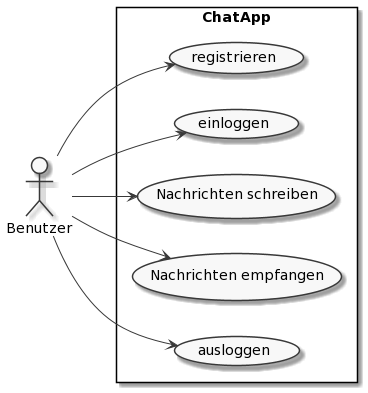
\includegraphics[width=0.7\textwidth]{Graphics/Usecase-Diagramm.png}
	\caption{Use-Case-Diagramm der ChatApp}
	\label{use-case}
\end{figure}

\section{Architekturentwurf}
Im diesem Abschnitt stellen wir die von uns entworfene Architektur vor und erläutern die wichtigsten Merkmale.
\subsection{Übersicht}
Wie in Abbildung \ref{entwurf} zu sehen ist besteht die Architektur aus einem Client mit graphischer Oberfläche (UI) einem API-Gateway, das alle Anfragen von Clienten empfängt und drei Microservices mit je einer eigenen Datenbank, die die Hauptfunktionalitäten des Systems implementieren.\newpage
\begin{figure}[bth] 
	\centering
	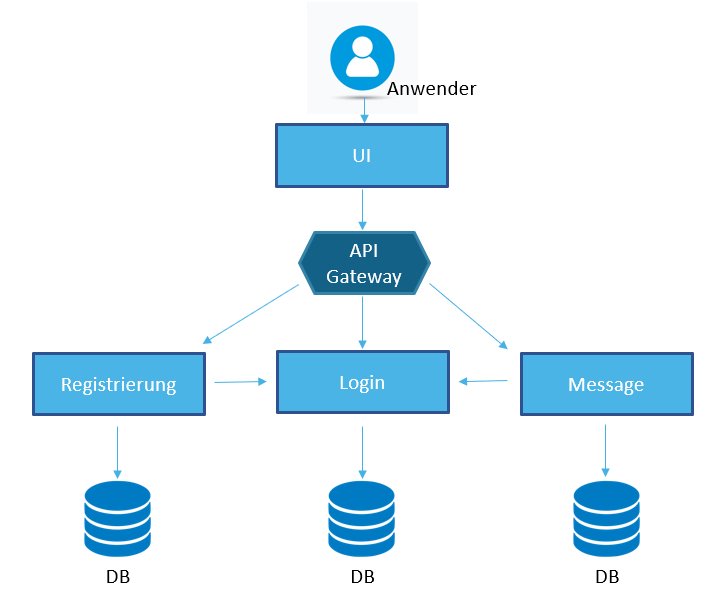
\includegraphics[width=0.6\textwidth]{Graphics/Architekturentwurf.png}
	\caption{Architekturentwurf der ChatApp}
	\label{entwurf}
\end{figure}
\subsection{Microservices}
Jede Funktion aus den Anforderungen korrespondiert mit einem Microservice. Die Aufteilung der Microservices ergibt sich aus der Annahme, dass die Funktionalitäten, die sie bereitstellen unterschiedlich oft genutzt werden: Anzahl der Registrierungen < Anzahl Login/Logout < Anzahl der geschriebenen Nachrichten/Abruf von Nachrichten). Daraus gewinnen wir eine individuelle Skalierbarkeit der Funktionen, ohne Redundanz.

\subsection{Registration-Microservice}
Über den Registration-Microservice kann sich ein Benutzer registrieren. Dazu stellt er eine Schnittstelle zur Verfügung an die man eine Nachricht mit E-Mail, Passwort und Land senden kann. Beim Eintreffen einer neuen Nachricht wird ein neuer Eintrag in seiner Datenbank generiert. Des Weiteren wird eine Nachricht an den Login-Service gesendet, mit der Anfrage, auch hier den neuen Benutzer anzulegen.

\subsection{Login-Microservice}
Der Login-Microservice stellt drei verschiedene Funktionen über eine Schnittstelle zur Verfügung: Anlegen eines neuen Benutzers, Einloggen und Ausloggen. Soll ein neuer Benutzer angelegt werden (dies wird vom Registration-Microservice angestoßen), so erzeugt der Microservice einen neuen Eintrag in der Login-Datenbank, in dem E-Mail (auch als ID verwendet) und Passwort des Benutzers gespeichert werden. Will sich ein Benutzer anmelden, gleicht der Microservice die Daten mit der Datenbank ab und stellt dem Benutzer, falls die Kredentialen korrekt waren, einen Token aus, welcher auch in der Datenbank gespeichert wird. Mit diesem Token, kann er sich dann bei anderen Microservices dann autorisieren. Meldet sich ein Benutzer ab, wird der Token einfach aus der Datenbank gelöscht.

\subsection{Message-Microservice}
Die Schnittstelle des Message-Microservices umfasst das Senden einer Nachricht und das Abrufen von empfangenen Nachrichten. Im Fall des Sendens müssen die folgenden Daten angegeben werden: eine Nachricht, eine Empfänger E-Mail Adresse und einen Token. Mithilfe des Tokens stellt der Message-Microservice sicher, dass der Sender eine gültige Session hat. Dazu sendet er eine entsprechende Nachricht an den Login-Microservice, der dann den Token bestätigt oder ablehnt. Im positiven Fall wird die Nachricht in der Datenbank des Microservices gespeichert. Will ein Benutzer seine Nachrichten abrufen, so muss er nur einen gültigen Token vorzeigen, den der Message-Microservice, wie beim Senden einer Nachricht, über den Login-Microservice abgleicht.

\subsection{API-Gateway}
Das API-Gateway schottet die Microservices ab. Das bedeutet, dass alle Anfragen vom Clienten nur an das API-Gateway gesendet werden und niemals direkt an die Microservices. Das Gateway leitet dann die Anfrage an den entsprechenden Mircoservice weiter und sendet dessen Antwort wieder an den Clienten. Die Abschottung hat mehrere Vorteile. Sicherheitsrelevante Aspekte wie z.B. DDoS-Protection oder der Schutz vor unbefugtem Zugriff (von Adressen, die nicht zum Client gehören) können auf das API-Gateway verlagert werden und müssen daher nicht in jedem Microservice implementiert werden.
Des Weiteren erfüllt das API-Gateway die Rolle eines Load-Balancers, der die Anfragen auf verschiedene Instanzen von Microservices verteilt. 

\subsection{Client (UI)}
Mithilfe des Clients können Anfragen an das System, genauer gesagt das API-Gateway, gesendet werden. Er enthält keine Funktionalitäten und dient lediglich zum Abrufen und Darstellen von Inhalten.

\begin{figure}[bth] 
	\centering
	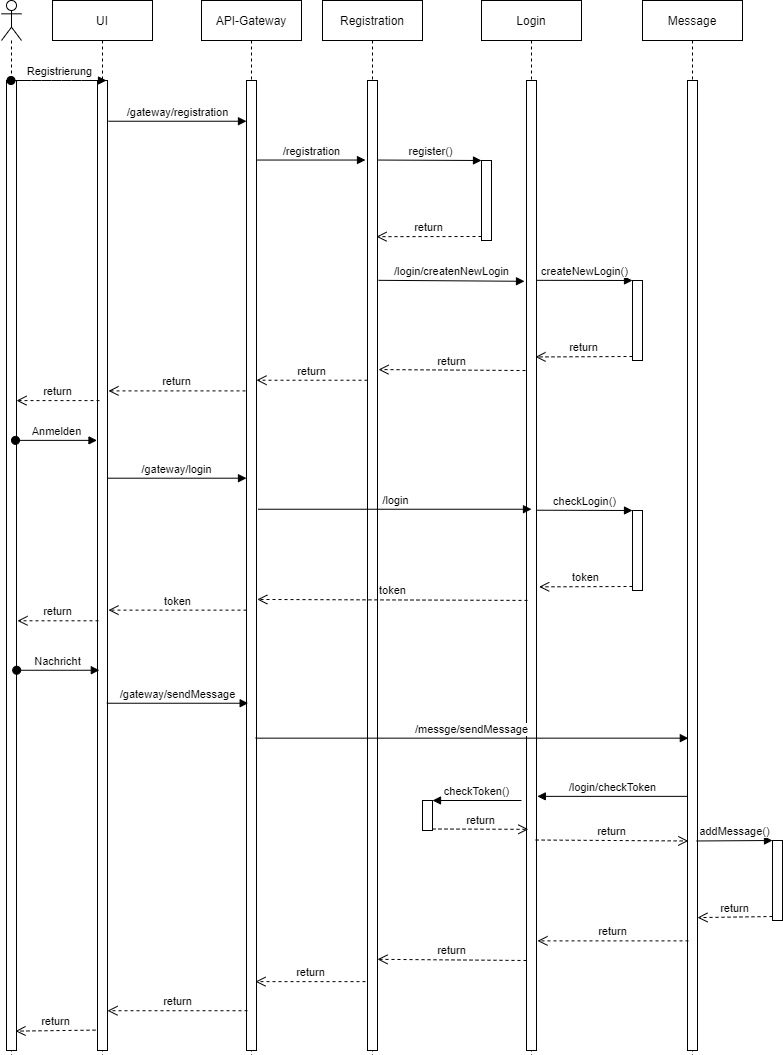
\includegraphics[width=1\textwidth]{Graphics/test2.png}
	\caption{Sequenzdiagramm}
\end{figure}

\subsection{Verbindungen zwischen Komponenten}
In Abbildung xx sind die drei wichtigsten Abläufe in einem Sequenzdiagramm festgehalten. Dargestellt sind die Registrierung, die Anmeldung und das Senden einer Nachricht. Es dient zum Verständnis der Zusammenhänge der einzelnen Komponenten.


\section{Implementierung des Prototyps}

In diesem Kapitel stellen wir unsere prototypische Implementierung vor. Das gesamte System ist in fünf Teile aufgeteilt (UI, API-Gateway, Registration-Microservice, Login-Microservice und Message-Microservice), wobei jeder Teil einem unabhängigem Projekt entspricht, aus welchem jeweils ein eigenständig ausführbares Programm entsteht.
Sämtliche Kommunikation wird über das HTTP Protokoll abgewickelt. Die Inhalte der Nachrichten sind dabei im \ac{JSON} Format.

\subsection{UI}
Die Benutzeroberfläche ist eine eigenständige React App. ReactJS ist eine Open-Source-JavaScript Bibliothek mit der Webanwendungen erstellt werden können.\\
Des Weiteren wurde zu dem HTML und JavaScript verwendet. HTML ist eine Auszeichnungssprache, die zur Strukturierung und Erstellung von Webseiten verwendet wird. JavaScript ist für das Verhalten und Aussehen einer Webseite zuständig.\\
Der Benutzer interagiert mit der ChatApp, indem er sich z.B. in der ChatApp registriert. Die Eingaben werden anhand von HTTP Requests an das API-Gateway geschickt, das die Daten zur Weiterverarbeitung an den entsprechenden Microservices weiterleitet. Empfange Daten werden ebenfalls von dem API-Gateway an die Benutzeroberfläche gesendet, sodass die ChatApp ausschließlich mit dem API-Gateway kommuniziert.

\subsection{API-Gateway}
Das API-Gateway ist mit Java und Maven als Build-Management-Tool implementiert. Es stellt eine HTTP Schnittstelle zur Verfügung, an die Nachrichten gesendet werden können, die es dann an die Microservices weiterleitet. Für das Gateway sind die Microservices ebenfalls über HTTP Schnittstellen erreichbar.
Das Loadbalancing ist für den Message-Microservice implementiert. Dabei kennt das API-Gateway zwei verschiedene Endpunkte unter denen jeweils eine Instanz des Message-Microservices auf Anfragen hört. Bekommt das Gateway eine Anfrage für den Message-Microservice wird abwechselnd eine der beiden Instanzen ausgewählt, an welche die Anfrage weitergeleitet wird. Die Wahl von zwei Instanzen ist hier zwecks Einfachheit gewählt. Es ist möglich mehr als nur zwei Instanzen des Message-Microservices oder eines anderen Microservices zu verwenden. Eine Möglichkeit um die Lastenverteilung zu Regeln wäre das Round-Robin-Verfahren, bei dem die Anfragen der Reihe nach auf die Microservices verteilt werden.

\subsection{Microservices}
Alle Microservices sind mit Java und Maven als Build-Management-Tool implementiert. Die Wahl der Programmiersprache und anderen Tools ist könnte dabei beliebig gewählt sein. Entscheidend ist nur die Schnittstelle die nach außen hin zur Verfügung stellt wird. Des Weiteren sind die Microservices Zustandslos. Für den Registration-Microservice und den Message-Microservice ist dies trivial, da sie sowieso keine temporären Daten speichern müssen. Der Login-Microservice muss sich jedoch den Token merken, den jeder Benutzer zur Autorisierung verwendet. Dies tut er indem er den Token in der Datenbank speichert.
Der Einfach halber wurden die Datenbanken für den Registration-Microservice und den Login-Microservice mit einfachen Java Klassen implementiert. Dies war aber für den Message-Microservice nicht möglich, da für ihn immer mindestens zwei Instanzen existieren, welche dann keine gemeinsame Datenquelle hätten. Um zumindest die Lösungsidee zu demonstrieren, haben wir eine einfache Datei als Datenbank verwenden, die für beide Instanzen immer zugänglich ist.